\section{Methods}\label{sec:project}

As already outlined in \autoref{sec:motivation}, we wanted to study the extent to which hate, discrimination and racism exist in German rap. In order to do so, we've used different methods of text analysis, which will be explained in more detail below. The described approach of our pipeline is also supplemented by a visual representation in \autoref{fig:pipeline}.

\begin{figure}[!htb]
  \centering
  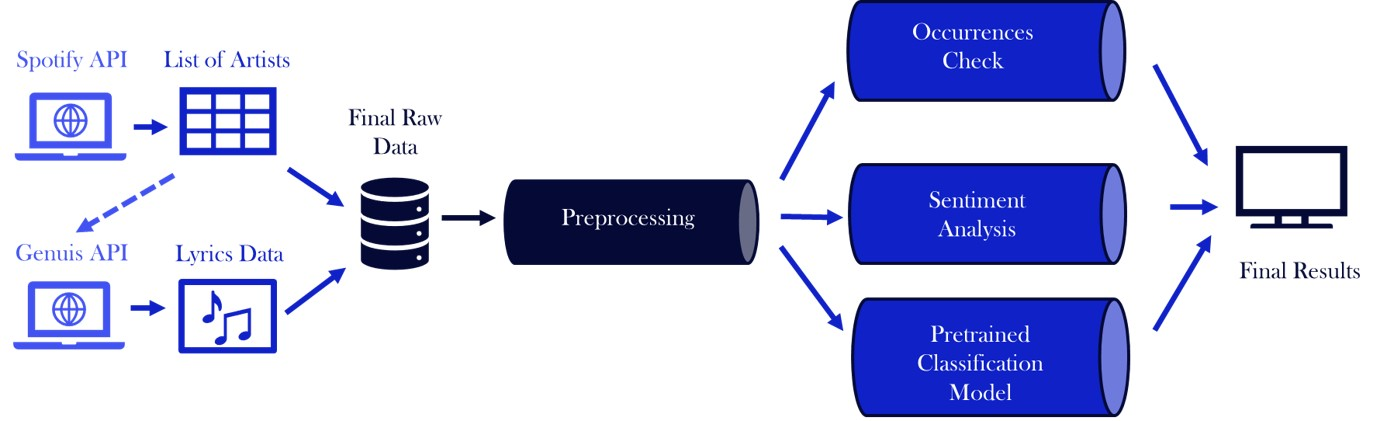
\includegraphics[width=\textwidth]{figures/pipeline.jpg}
  \caption[]{Text Analytics Pipeline}
  \label{fig:pipeline}
  \end{figure}

  Our pipeline can be split into the following stages. Details regarding the individual points are detailed below:
  \begin{enumerate}
    \item Data acquisition
    \item Preprocessing
    \item Text analysis methods: Occurrences check, Sentiment analysis, Zero-shot classification
  \end{enumerate}

\subsection*{Data acquisition}

Since the subject of interest for our project was the analysis of German rap texts, we first needed to gather a dataset of German rap lyrics. We've decided to start with obtaining a list of German rap artists from the most popular German rap playlists on Spotify between the years 1998 and 2022. This was done with a Python library called spotipy \cite{spotipy}, which works with the Spotify API.

For our analysis to have a meaningful interpretation of German rap's influence on German society, we decided to scrape the 15 most popular songs by each artist. In addition to the lyrics, we also saved relevant information that could be useful in later parts of the analysis. This information included the album to which a song belongs, the song's date of release, featured artists, etc.

To acquire this information, we've decided to use Genius \cite{genius}, a website which provides a vast amount of lyrics for many songs. Genius offers their own API which allows for scraping of lyrics. In addition, the API has a Python library to work with. However, this API has different limitations regarding the amount of songs allowed to be scraped per artist, as well as the available information for the songs. 

In order to overcome those limitations, we partly used the Genius API and the BeautifulSoup library \cite{beatifulsoup}. This also allowed us to speed up the scraping process by using multi-threading, which wasn't possible with the API due to limitations on the amount of requests allowed at a given moment. The initial resulting dataset contained about 10,500 German songs from about 800 artists.

\subsection*{Preprocessing}

After scraping, the resulting dataset needed to be preprocessed. Many of the songs we've scraped contained annotations for the different parts of the songs, such as the different verses and the chorus. These annotations sometimes also included the names of the artists in the case of having multiple of them in one song. Those parts were usually given by brackets, e.g. [Chorus] or [Verse 1], which made it easier to remove. Furthermore, many songs contained commas and points in places where they don't belong, or sentences that were cut by an additional line. We've used Python's Regular expression library (regex) to take care of the bracketed parts and the additional unwanted punctuation.

Upon inspection of the different scraped songs, we noticed that our dataset contained some songs for which the German language wasn't the major language. In fact, some of the songs didn't contain German words at all. For our analysis, it was crucial to filter out those songs. To do so, we could benefit from the Polyglot library \cite{polyglot}, which helped us to remove undesirable songs. This step reduced our dataset to about 5992 songs.

For further preparation of the dataset for the analysis part, we had to get rid of stopwords and lemmatize the text. For the removal of stopwords, we were faced with several lists of stopwords for German language ranging from about 300 words to 1500+ words \cite{stopwords1}. The different stopwords lists offered different advantages and disadvantages. For example, removing critical information versus keeping information that may not contribute or even undermine the success of the analysis. We've eventually decided to work with the stopwords list built by Gene Diaz \cite{stopwords2}, which has about 620 stopwords. For the lemmatization part, we've used the 'de\_core\_news\_sm' model from NLP framework spaCy \cite{spacy}.

A substantial issue, which could have posed lots of implications and possibly prevented us from being able to correctly analyze the texts, was the lack of punctuation in the vast majority of the songs. We wanted to be able to break down the songs into meaningful sentences that could be processed and analyzed. To solve this issue, we've used a punctuation restoration library called 'Deep Multilingual Punctuation Prediction' \cite{auto-punctuation}. This is a NLP model which was made for restoring punctuation of transcribed spoken language and was trained on the Europarl dataset \cite{europarl}.

\subsection*{Text analysis methods}

\subsubsection*{Occurrences check}

One big point of interest we wanted to investigate was the changes in trends and narratives over time in the German rap genre, as already discussed by Puls magazine and Spiegel magazine (see \autoref{sec:research}).

We've decided to carry out an occurrence check on specific words in the songs and to roughly label songs using those occurrences to draw conclusions. Firstly, dictionaries with positive and negative sentiments were manually created for each of the following labels : Homophobia, misogyny, anti-disability, anti-semitism, racism, violence, love and grief. The last two categories were added to provide adequate comparability of the results with respect to the other categories.

Due to the fact that those dictionaries were manually created by us, we couldn't catch all possible synonyms and related words for each label. To overcome this, initial words were given for each category and synonyms were searched via Word2Vec model and its built-in k-nearest-neighbour method. A pre-trained model by Andreas M{\"u}ller \cite{mueller2015} served as a basis. This model is built on texts from the German pages on Wikipedia and German news platforms. This causes certain complications, as the base corpus of M{\"u}ller only partially corresponds to the language used in rap genre and particularly excludes vulgar words.

Accordingly, we had to manually adjust and correct the resulting dictionaries, which were selected on the basis of the 20 closest neighbours of the given input words. 

In order to determine the specific occurrences of the given categories in the lyrics, all lyrics were checked against all dictionaries of the categories. We allowed substrings of the matching pairs in a certain way: If one of the words from the lyrics started or ended with a term from a category dictionary, this was counted as an occurrence. Likewise, an occurrence was counted if at least 75\% of a word from the lyrics was identified as a substring in a corresponding word from a category dictionary.

\subsubsection*{Sentiment analysis}

In addition to that counting analysis, we wanted to look for different pre-trained classification models to include the power of advanced natural language processing tools to enrich our analysis. To do this, we looked for models that could classify the sentiment of the songs in the context of our research questions. We found two different, BERT \cite{bert} based models which we could apply to our data: 'German Sentiment Bert' \cite{gbert} by Oliver Guhr and 'German Toxicity Classifier Plus V2' \cite{toxicity} by Elisei Stakovskii.

The 'German Sentiment Bert' classification model was trained on 1.834 million German samples and outputs the probabilities for the three classes 'negative', 'neutral', 'positive'. For every song, we predicted the probability of each line and mapped it from -1 (negative) to 1 (positive) where 0 is neutral. More specifically, for each line, the probability of the highest class was extracted and multiplied by the previously mentioned values -1 (negative), 1 (positive) and 0 (neutral). We subsequently summed up these values across the entire song and divided it by the number of lines to get the average sentiment of the total song.

The 'German Toxicity Classifier Plus V2' model was trained for toxicity labeling on the classes 'toxicity' and 'neutral'. Author Elisei Stakovskii built this model by fine-tuning the 'German BERT model' of MDZ Digital Library team at the Bavarian State Library. For the toxicity classifier, we processed the songs in the same manner as we did for the German Sentiment Bert model: we predicted the lines of each song, then summed the results up and averaged them. We again wanted to have a continuous mapping, which we defined as -1 to be not toxic and 1 to be toxic. For each line, we therefore took the most prominent class and multiplied it by -1 if it was 'neutral' and by 1 if it was 'toxic'.

\begin{comment}
This model helped us to get further insights on the texts and managed to capture the sentiment of songs beyond them being positive or negative. Some sentences can be intreperted by the sentiment model as negative, but as neutral by the toxicity model. We will discuss later on the correlation between those two in the evaluation part.
\end{comment}

\subsubsection*{Zero-shot classification}
For this purpose, we decided to use a zero-shot classifier \cite{zero-shot}. A zero-shot classifier is an NLP model that receives as input a sentence, a question about that sentence, and a list of labels to which the model should assign the sentence depending on the input question. The model used is based on the XLM-RoBERTa model \cite{roberta} and was then refined for the classification task. The model allowed us to create our own labels and predict the probabilities for a given sentence based on our own labels. For our task, it was sufficient to define the question: "What is this example about?". At first, we tried to use only the labels we were already interested in, namely 'homophobic', 'racist', 'misogynist', 'anti-semitic', 'violent', 'beautiful' and 'sad'. 

However, we noticed that the model might misclassify a sentence if none of the labels fit exactly. This is due to the fact that it has no choice other than to assign the sentence to one of these labels. Therefore, in addition to our original labels, we decided to add some labels that can be used as offset labels, so the model can choose to use labels other than the labels we are interested in. Thus, the model does not always have to choose a label that is not necessarily the best fit. For example, in order to improve the quality of the classifier, we used the label "neutral" in this specific way. Finally, a sentence that is neither sad nor beautiful is not necessarily assigned to the other negative labels, such as anti-semitic or misogynistic.

For the concrete classification of the songs, we followed the same approach as for the sentiment analysis. The preprocessed lines of each song were analysed via zero-shot classifier and the probabilities of the categories 'homophobic', 'racist', 'misogynist', 'anti-semitic', 'violent', 'beautiful', 'sad', 'lovely' and 'neutral' were determined. We took the average of these probabilities across all lines of each song. Thus, we obtained a distribution for probabilities of the described categories of a whole song.

